\documentclass[12pt, a4paper]{article}
% \usepackage{mathtools}
\usepackage{graphicx}
\usepackage{amsthm}
\usepackage{hyperref}
\usepackage{amssymb}
\graphicspath{{images/}}

\hypersetup{
    colorlinks=true,
    linkcolor=blue,
    urlcolor=cyan
}

\title{AP Macroeconomics Notes}
\author{Franklin Chen}
\date{22 Feburary 2024 - 21 May 2025}

\theoremstyle{definition}
\newtheorem{definition}{Definition}

\begin{document}
\maketitle
\newpage
% comment

\tableofcontents

\newpage

pro tip: any economic term with "real" = adjusted for inflation.

\section{Intro to Economics}
Corresponds to Chapter 2: "The Discipline of Economics."

\subsection{What is Economics?}

\begin{definition}[Economics]
    The study of resources and how to optimally use resources.
    Often to answer the question "Should we do \textit{A} or \textit{B} with this limited resource?"
\end{definition}

In this context, the word "resource" has a specific meaning.

\begin{definition}[Resource]
    Anything that can be used to produce a good or service.
    Every resoruce is classified into one of three categories:
    \begin{itemize}
        \item \textbf{Land}: natural resources. (Eg. crude oil, farmland, oceans)
        \item \textbf{Labor}: work people do to produce goods and services. (Eg. physical labor like building or sports, mental labor like professors)
        \item \textbf{Capital}: equipment used to produce goods or more resources. (Eg. factories, computers)
    \end{itemize}
\end{definition}

Economics is broken into two fields: \textbf{microeconomics} and \textbf{macroeconomics}.

\begin{definition}[Microeconomics]
    The study of economic problems faced at the individual level; individuals, families, and firms.
    Eg. "does this particular family save enough to provide for its future needs?"
\end{definition}

\begin{definition}[Macroeconomics]
    The study of economics problems faced at the national level; states, countries, and internationally.
    Eg. "should we allocate resources from national defense to education?"
\end{definition}

Sometimes, we may discuss \textbf{positive economics}: the scientific analysis of economics via the hypothesis-test-conclusion model.
Alternatively, we may discuss \textbf{normative economics}: the ethical analysis of economics- the way things \textit{should} be.

\subsection{Opportunity Cost and the PPF}

\begin{definition}[Opportunity Cost]
    The potential benefit lost from choosing one alternative over the other.
    For example, when you spend two hours studying, you lose two hours of relaxation.    
    Gains of the option not chosen - gains of the opportunity chosen = opportunity cost.
\end{definition}

In macroeconomics, opportunity cost is often quantative.
If a nation decides to spend more resources to produce a good A, they will "lose" the good B that could have been produced with the same resources.

\begin{figure}[ht] % h = where it appears in text
    \centering
    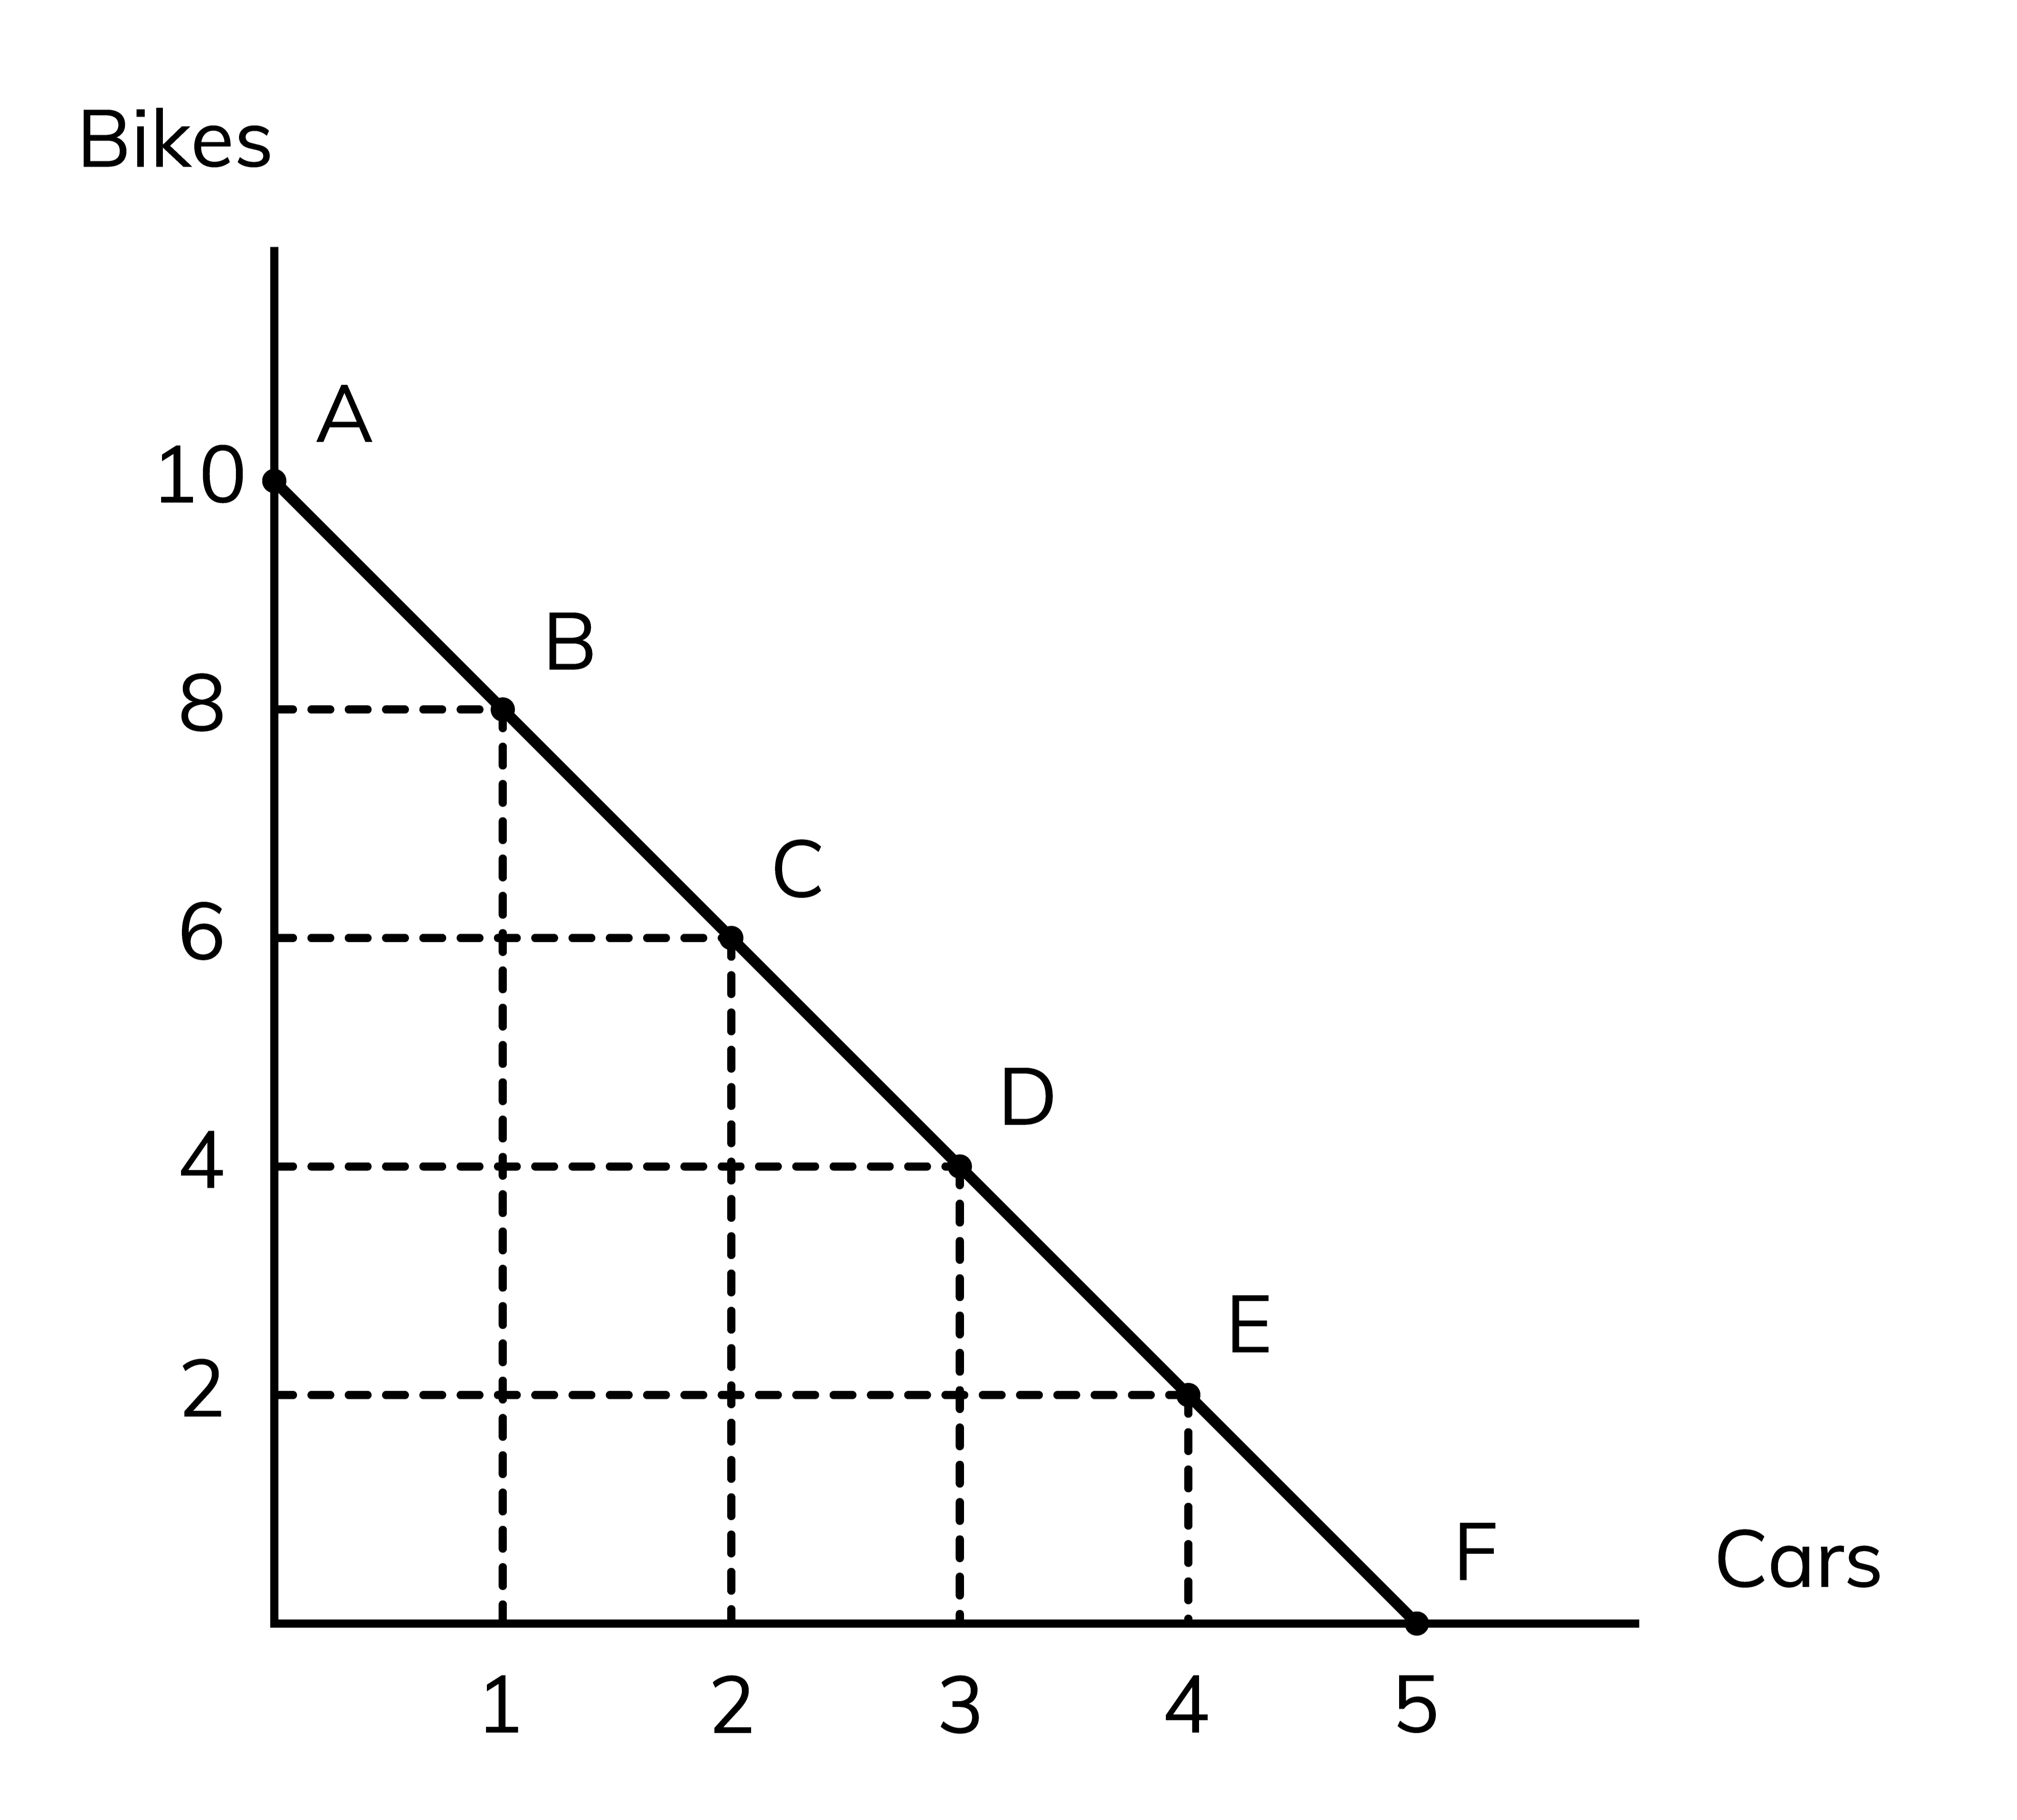
\includegraphics[width=0.75\textwidth]{ppf.png}
    \caption{A Production Possibilties Frontier (PPF) showing a hypothetical nation's possible production of bikes and cars.}
    \label{fig:ppf}
\end{figure}

For example, consider Figure \ref{fig:ppf}.
In this case:

\[\textrm{Opportunity Cost of Bikes} = \frac{\textrm{Change in Car Production}}{\textrm{Change in Bike Production}} = 0.5 \textrm{cars}/\textrm{bike}\]

The opporutnity cost of cars is the reciproical of the opportunity cost of bikes: that is, 2 bikes/car.

Figure \ref{fig:ppf} is a \textbf{production possibilties frontier}: it shows all the combinations of the goods that can be produced if the economy uses all of its resources fully and \textbf{efficently} (to their maximum potential).
\textit{All points on the curve are optimal; a normative analysis is required to determine what point is preferred.}

Points "inside" the PPF are possible, but aren't optimal. (This may occur due to environmental, labor or other restrictions.)
Points "outside" the PPF are currently impossible: resources can't be used efficently enough to reach that point.

The PPF may shift for two primary reasons: changes in the \textit{amount of resources} or \textit{productivity/technology}.
Increasing the amount of resources or improving technology used to produced said resources would shift the PPF to the right.
Similarly, decreasing the amount of resources or somehow regressing in technology (war/disaster) would shift the PPF to the left.


\subsection{Laws of Costs}
Often, PPFs aren't straight lines; the opportunity cost varies depending on the current amount being produced.
More often, the opportunity cost of each extra product increases per product already produced.
Graphically, this causes a PPF concave to the origin.
This is known as \textbf{the law of increasing costs}.

Generally, the law of increasing costs happens as people less and less in tune with producing a good are hired to produce it.

Alternatively, the inverse may happen: the opportunity cost of each extra product may decrease per product already produced.
This may happen as more infrastructure is put into place, it takes less resources to produce each unit good.
This causes a PPF convex to the origin, and is known as \textbf{the law of decreasing costs}.

\subsection{Absolute and Comparitive Advantage}
\begin{definition}[Specialization]
    When an entity focuses on the production of a limited scope of goods for greater efficency.
\end{definition}

It can be shown that dividing labor into specialized tasks could increase productivity and output, \textit{even at the national scale.}

\begin{figure}[ht] % h = where it appears in text
    \centering
    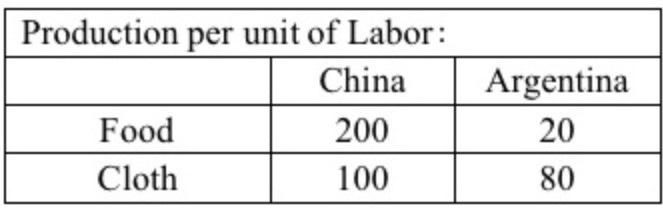
\includegraphics[width=0.75\textwidth]{advantage.jpg}
    \caption{A hypothetical example of production costs of food and cloth in China and Argentina.}
    \label{fig:advantage}
\end{figure}

Consider Figure \ref{fig:advantage}. 
In this case, China has the \textbf{absolute advantage} in both food and cloth because China can produce both more efficently than Argentina.
However, Argentina has the \textbf{comparitive advantage} in cloth, because it has a lower opportunity cost (0.25 food/cloth vs. 2 food/cloth).
Similarly, China has the comparitive advantage in food (0.5 cloth/food vs. 4 cloth/food).
It can be shown that by specializing in the good a nation has a competitive advantage of, the maximal amount of goods will be produced between the two nations.

Supposing that countries only produce their competitive advantage good, an optimal trading ratio to benefit both countries can be found by considering opportunity cost.
Trading x units of food for y units of cloth would be optimal if x/y is less than the opportunity cost of cloth in China (2 food/cloth) and y/x is less than the opportuntiy cost of food in Argentina (4 food/cloth).
For example, trading 1 unit of food per 1 unit of cloth would benefit both countries, as it is less than both of the countries' individual opportunity costs.

\newpage

\section{Economic Systems}
Corresponds to Chapter 3: "Economic Systems."

Economics deals with three primary problems:
\begin{itemize}
    \item How much, if any, of each good and service should be produced?
    \item Who will get how much of each good and service?
    \item How should these goods and services be distributed?
\end{itemize}

While these problems may be easy to answer for small systems, these problems become exponentially harder to deal with as the size of the economy grows.
Note the idea of opportunity cost (producing something will reduce production of other products) 
and \textit{related costs}: producing more of a product will require more production of capital.

For example, producing more food may take away money from the cosmetic industry; opportunity cost; and require the production of more tractors and farm equipment; related costs.

Societies tackle this problem in three ways: \textbf{command economies}, \textbf{capitalism}, or a mix of the two.
These can be viewed as a spectrum: command economies on one end, and capitalism on the other.

\subsection{Command Economies}
\begin{definition}[Command Economy]
    Also referred to as "communism" or "socialism."
    An economy in which the government determines what will be produced, how much will be produced, and who recieves the products.
\end{definition}

Command economies use quotas and production plans to dictate how much of each good or resource is produced. 
By setting prices on goods and services and controlling the wage rates of almost all citizens, the government is able to control the access to products.

Due to how interconnected individual goods and services are with one another, it is nearly impossible to perfectly coordinate production requirements.
Many quotas may fail if a "requirement" quota fails to be met.
Additionally, incentives to work hard and innovate are discouraged, as there is little benefit for doing so.

However, command economies can also artificially change prices; ex. artificially lowering the price of textbooks to encourage education.
Additionally, fixed wages can eliminate the lower class.

Two examples of countries with command economies are Cuba and North Korea.

\subsection{Capitalism}
\begin{definition}[Capitalism]
    Economic system where supply and demand determine prices.
\end{definition}

In a capitalist economy, the \textbf{consumer} dictates the production of goods.
For example, if consumers want more of a certain product, the purchases of that product will go up.
This signals to producers to increase the production of that product (often cutting something else in the process).

An individual's income determines how much of the net production they will recieve.
Income is also another variable within such an economy (the price of labor).

In a purely capitalist economy, the government has no direct influence.
However, in practice, no country is purely capitalist: the government often needs to step in when the economy won't equitably provide important resources, like food or higher education.

\subsubsection{Allocative Efficency}
\begin{definition}[Allocative Efficency, the "invisible hand"]
    When resources are deployed to produce just the right amount of products to satisfy society's wants.
\end{definition}


When prices are determined by a capitalist economy, \textbf{allocative efficency} is achieved.
The capitalist economy is able to answer the critical questions of economics in a \textit{decentralized} way (with no ruling body).
Products and quantity are determined by the consumer, as mentioned before.
Who recieves goods is also answered, as the price of labor will reward those who appeal to consumer wants.

\subsection{The Circular Flow Diagram}

\begin{figure}[ht] % h = where it appears in text
    \centering
    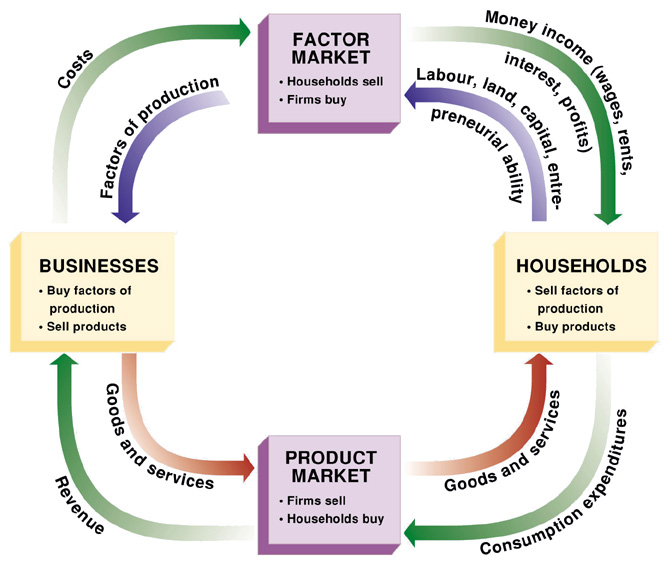
\includegraphics[width=0.75\textwidth]{circular flow.jpg}
    \caption{The Circular Flow Diagram.}
    \label{fig:cfd}
\end{figure}
In capitalist economies, most of the resources are "owned" by individuals and households;
via stockholders "owning" companies and government facilites being "owned" by everybody.

\begin{definition}[Market]
    A mechanism that allows buyers and sellers to exchange a good or service.
\end{definition}


The \textbf{circular flow diagram} (\ref{fig:cfd}) shows how resources are flow from households to firms in exchange for wages.
This trade of resources for money is known as the \textit{market for resources} or \textit{factor market}.
Households spend their income to purchase goods and services supplied by firms: the \textit{market for goods and services} or \textit{product market}.


\newpage

\section{Supply and Demand}
Correpsonds to Chapter 4: "Demand and Supply: The Basics."

\subsection{Demand}
\begin{definition}[Demand]
    The quantity of a product a consumer is willing and able to purchase at each and every prices.
    The demand for a product is shown graphically as a demand curve.
\end{definition}

\begin{definition}[Law of Demand]
    Holding all else equal (\textit{ceteris paribus}), if the price of a product increases, the quantity demanded decreases and vice versa.
    Equivelently, the slope of a demand curve is always negative.
\end{definition}

There are three major reasons for why the Law of Demand happens:
\begin{enumerate}
    \item \textbf{The Income Effect}: When prices fall, consumers can afford to buy more of a product, and vice versa. The \textit{purchasing} power of the consumer decreases as the prices increase.
    \item \textbf{The Substitution Effect}: If a substitute for a good exists, an increase in price for the good will lead to more demand for the alternative and thus less demand for the original good.
    \item \textbf{Diminishing Marginal Utility}: As more units of a product are "consumed" the \textit{utility} or satisfaction from each individual product decreases. As utility decerases, so does the price the consumer is willing to pay.
\end{enumerate}

\begin{figure}[ht] % h = where it appears in text
    \centering
    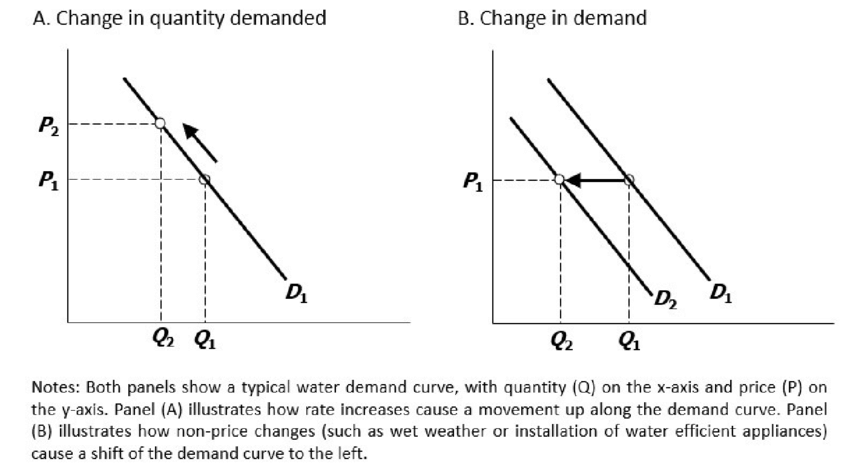
\includegraphics[width=1\textwidth]{demand.png}
    \caption{Demand curves.}
    \label{fig:demand}
\end{figure}

\subsubsection{Changes in Demand and Quantity Demanded}
\begin{definition}[Quantity Demanded]
    The quantity of a product demanded at \textbf{one} specific price.
    When \textbf{only the price} of a product changes, the quantity demanded will change.
    This is the movement of a point along a \textbf{constant} demand curve.
\end{definition}

An increase in demand leads to a shift to the right, VV.

On the other hand, if the \textbf{determinants of demand} change, then the demand curve \textit{will} shift the curve to the left or right.
The determinants of demand are as follows:

\textbf{Substitute Goods} are two goods that are interchangable- see the substitution effect.
When the price of the original good goes up, the quantity demanded for the original good decreases and the demand \textit{curve} of the substitute good will go outwards, thus resulting in a shifted quantity demanded.

\textbf{Preferences} refer to consumers' tastes or preferences for a good or service.
If people's desire for a product increase, then the demand curve will shift to the right, and vice versa.

\textbf{Population} refers to the total number of buyers in a specific market.
Bigger market = more demand = shift to the right.

If a consumer's \textbf{income} increases, their demand for all products will generally increase.
Most goods are \textit{normal goods} (income increases = demand for good increases), but some may be \textit{inferior goods} (income increases = less demand).
Think of normal goods like superior proudcts (new car, new clothes) and inferior goods like poor products (used cars, second-hand clothes).

\textbf{Complementary Goods} are goods that are purchased seperately but used together.
When the demand for the original good goes up, so will the demand for the complementary good, and vice versa.
Like the opposite of substitue goods.

\textbf{Expectations} of higher prices will increase the current demand before the price increases.

Remember the acronym SPICE:
\begin{itemize}
    \item \textbf{S}ubstitute Goods
    \item \textbf{P}references and \textbf{P}opulation
    \item \textbf{I}ncome
    \item \textbf{C}omplementary goods
    \item \textbf{E}xpectations
\end{itemize}

\subsection{Supply}
Similar to consumers, suppliers also have their own \textbf{supply} curves.

\begin{definition}[Supply]
    The quantity of product a supplier is willing and able to produce or put on sale at each and every price.
    The supply for a product is shown graphically as a supply curve.
\end{definition}

\begin{definition}[Law of Supply]
    Ceteris paribus, if the price of a product increases, the quantity of product a supplier is willing to provide increases.
    Equivelently, the slope of a supply curve is always positive.
\end{definition}

The Law of Supply happens for two major reasons:
\begin{enumerate}
    \item Greater price = more profit. yeah thats it
    \item As producers increase production, the marginal cost of producing each product increases, requiring higher prices to justify producing a higher quantity of product.
\end{enumerate}

\subsubsection{Changes in Supply and Quantity Supplied}
\begin{definition}[Quantity Supplied]
    The quantity of a product produced at \textbf{one} specific price.
    When \textbf{only the price} of a product changes the quantity produced will change.
    This is the movement of a point along a \textbf{constant} supply curve.
\end{definition}

Yet again, there exist \textbf{determinants of supply}.
Note, in this case, an increase in supply would lead to a \textit{shift to the right}- more quantity for less price. VV.
The determinants of supply are as follows:

\textbf{Resource costs and availability}: when the cost of producing a product increases, the supply of that product will decrease, VV.
When one of the resources (land, labor, capital) used in production changes in price, supply will change.

\textbf{Alternative Prices}: sometiems, a firm can easily switch between several different products.
In some cases, it may be better to produce more of another product to maximize profit.
Thus, the prices of alternative prices will affect the supply of both.

New \textbf{technology} can decrease production costs and increase productivity, resulting in greater supply.

\textbf{Taxes} on the production of a good will result in increased production costs, decreasing supply.
Alternatively, a \textbf{subsidy}- payment from the government to produce a product- will increase profits at all levels and increase supply.

Similar to consumers, if producers \textbf{expect} higher prices in the future, they may hold back the amount produced, decreasing current supply for the ultimate goal of increasing profits in the future.
VV.

A greater \textbf{number of sellers} increases net supply.
While the extra competition may decrease the supply for an individual seller, the result is a greater supply overall.
This is usually good for consumers, who recieve more choice and lower prices as the suppy curve shifts to the right.

Remember the acronym ROTTEN:
\begin{itemize}
    \item \textbf{R}esource costs and Availability
    \item \textbf{O}ther good's prices
    \item \textbf{T}ncome
    \item \textbf{T}axes and Subsidies
    \item \textbf{E}xpectations
    \item \textbf{N}umber of sellers
\end{itemize}

\subsection{Market Equilibrium}

At the point where the supply and demand curve intersects, there exists \textbf{market equilibrium}: consumers want the exact amount that producers want to produce.
This is also known as the \textit{market-clearing price}.
Otherwise, there is \textbf{disequilibrium}: the market is sub-optimal for consumers and producers.

A \textbf{surplus} exists if supply outweighs demand, resulting in lower prices and thus lower supply.
A \textbf{shortage} exists if demand outweighs supply, resulting in higher prices and thus higher supply.
In a perfectly competitive market, both scenarios will eventually converge back to equilibrium.

\subsubsection{Changes in Equilibrium}
Questions may ask about an equilibrium price after a supply and/or demand shift.

To solve these, first consider what curve the shift is affecting: supply, demand, or both?
Then, consider whether if it is an increase (right) or decrease (left), and then shift the curve, noting the new equilibrium.
Generally, shifts should follow the following table.
If in doubt, draw a picture of supply and demand.


\begin{figure}[ht] % h = where it appears in text
    \centering
    \begin{tabular}{ |c|c|c|c| } 
        \hline
        Change & Shift & Eq. Price & Eq. Quantity  \\
        \hline
        Supply Increase & Supply Right  & Down  & Up   \\
        Supply Decrease & Supply Left   & Up    & Down \\ 
        Demand Increase & Demand Right  & Up    & Up   \\ 
        Demand Decrease & Demand Left   & Down  & Down \\
        \hline
    \end{tabular}
    \caption{Table of both supply and demand shifts and effects.}
    \label{fig:shifts}
\end{figure}

\subsubsection{Double-Shifts}
Occasionally, questions may be asked where there are simultaneous shifts in both demand and supply.
\textbf{For the purposes of AP Macroeconomics, you will NOT need to calculate exact double-shift equilibrium values.}
Therefore, some values will be indeterminate- see the table below.

\begin{figure}[ht] % h = where it appears in text
    \centering
    \begin{tabular}{ |c|c|c|c| } 
        \hline
        Demand & Supply & Eq. Price & Eq. Quantity  \\
        \hline
        Increase & Increase & Indeterminate & Increase      \\
        Decrease & Decrease & Indeterminate & Decrease      \\ 
        Increase & Decrease & Increase      & Indeterminate \\ 
        Decrease & Increase & Decrease      & Indeterminate \\
        \hline
    \end{tabular}
    \caption{Table of simulatenous supply and demand shifts and effects on equilibrium.}
    \label{fig:dshifts}
\end{figure}

\newpage

\section{Gross Domestic Product}
Corresponds to Chapter 12: "The National Economic Accounts."

\subsection{What is GDP?}
\begin{definition}[Gross Domestic Product (GDP)]
    A measure of the dollar value of production within a nation's borders.
    Generally speaking, bigger GDP = healther economy.
    For 2021, USA's GDP was estimated around \$23.0 trillion.
\end{definition}

Broadly speaking, GDP can be calculated as follows:
\begin{enumerate}
    \item A representative surveys the major suppliers and retailers of a product.
    \item Through this survey, an estimate for the total number of products produced and their average value is obtained.
    \item Number of products produced $\times$ average product price $\approx$ GDP for that specific product.
    \item Total GDP = $\sum$ GDP for all products
\end{enumerate}

In step (3), only considering the total number of products \textit{sold} yields the \textit{final sales} metric.
This is \textbf{NOT} the GDP.

\subsection{Estimation Techniques}
In practice, there are many complications with the process discussed above.
Different estimation techniques account for these complications, but often introduce their own flaws.
In theory, all estimates should have the same value, but this is often not the case.

\subsubsection{Expenditures}
Rather than considering individual products, the \textbf{expenditure} approach breaks down GDP into several expenditure categories, which are calculated individually and summed together.

\begin{itemize}
    \item \textbf{Consumption Expenditures} refer to all the goods and services produced and sold to households.
    \item \textbf{Government Expenditures} refer to all goods and services produced and sold to local, state, and federal governments. Governments often buy products that households will not (eg. fighter jets) or products in quantites that differ from households (eg. high-end computers)
    \item \textbf{Investment Expenditures} (sometimes just "investment") refer to all capital goods and services, including plants, equipments, residential construction, and final sales (see section 4.1). This category mainly consists of independent companies/firms.
    \item \textbf{Exports and Imports}: many goods may be produced here and sold abroad, or goods may be purchased from abroad. As imports are produced outside a country's borders (not part of GDP), imports are subtracted from exports to get \textit{net exports}.
\end{itemize}

The expenditure approach to GDP is summarized with the following formula:

\[\textrm{GDP} = C + I + G + X\]

where C = consumption expenditures (by households), I = investment expenditures (by firms), G = government expenditures, and X = "net exports" = exports - imports.
Often, a majority of GDP comes from consumption expenditures (70\% in 2021).

While this formula appears simple, note that calculating even one of these variables requires significant effort and time.

\subsubsection{Income}

The revenue gained by producing a product is distributed between the different producers of that product: often including labor, materials, overhead (utility companies), and the producer company.
Obviously, the revenue gained by all parties would be just enough to buy that product back.
Therefore, in theory, GDP can be calculated by considering \textbf{the total income of the economy} instead- the \textbf{income approach}.

Wages and salaries are the predominant type of income.
Other types of income include:
\begin{itemize}
    \item Proprietors' income: income earned by self-employment or unincorporated buisnesses (???)
    \item Rental income: income from the use of occupation or porperty (renting stuff)
    \item Interest income: income from bank interest lmao
    \item Corporate profits: income gained by companies that are distributed to its shareholders
\end{itemize}

Some adjustments need to be made once the total is summed- notably, indirect buisness taxes (ex. buisness licenses), depreciation, and other miscallenous items must be accounted for.

\subsubsection{Value-Added}

The \textbf{value-added approach} considers what producers and industries add "value" to the final retail price.

Consider a producer gathering raw uranium, enriching it, and selling it to a nuclear reactor for (hypothetical) \$10.
The nuclear reactor uses this refined uranium to generate power, which is sold to customers for (hypothetical) \$15, adding \$5 of value in the process.
The GDP in this scenario is calculated by adding the value of the uranium at each stage of the process: \$0 (raw uranium) + \$10 (refined uranium) + \$5 (power).

While the U.S. does not use the value-added approach in the BEA (see National Accounts), other countries often use this approach to estimate GDP and set taxes at each stage of production.

\subsubsection{Real GDP}

GDP itself \textbf{DOES NOT} account for price changes.
Simply because this year's GDP was greater than last year's GDP does NOT imply that we produced more this year: prices could have simply risen higher than last year.

To account for this, \textbf{real GDP} (or "constant-dollar") is calculated using the prices from a \textbf{base year}.
It doesn't matter which year is chosen as the base; it ensures that all prices are held constant, such that any changes are due to a change in production alone.
(To differentiate, regular GDP may be referred to as "nominal" or "current-dollar" GDP.)

\subsection{Other GDP Factors}

\subsubsection{The Underground Economy}
\textit{The underground economy} refers to goods and services not counted in GDP- anything that does not pass through a market.
This obviously includes illegal activity (drugs, bribes, etc...), but also undocumented activites, notably any activies that households do for themselves.

This accounts for a significant amount of GDP, and some sources say that it can account for more than 50\% of GDP.

\subsubsection{Per Capita GDP}
While Japan and Montana are the same size, they have vastly different GDP's.
This is mainly due to population- the population of Japan is about 128 times that of Montana.

To compare which has a "higher standard of material well-being," divide the GDP by the population to get the \textbf{Per Capita GDP.}

\subsubsection{Limitations of GDP}
GDP is used as the primary measure of a country's quality of life.
However, it's not perfect: GDP does not account for social factors (war, class inequality, traffic, etc...) or where products go (possibly to a few select families).

\subsection{National Economic Accounts}
The \textbf{National Economic Accounts (NEA)} make up a comprehensive group of statistics that measure various aspects of the economy's performance.
Notably, the NEA tracks many measures of income and production, including GDP.
The NEA provides estimates for the USA's GDP using all the estimation techniques discussed above, providing relevant substatistics.
Updates are published under a periodical titled "Survey of Current Buisness," and are available online at the home page of the \textit{Bureau of Economic Analysis} (BEA), an agency within the Department of Commerce.

The BEA provides "flash" updates for GDP each quarter, about 30 days after the quarter ends.
Annual estimates of GDP are much more reliable, but they too are subject to revision.

\newpage

\section{Inflation and Unemployment}
Corresponds to Chapter 13: "Inflation and Unemployment."

\newpage

\section{Money and Banking}
Corresponds to Chapter 14: "Money and Banking"

\newpage

\section{Monetary Theory}
Corresponds to Chapter 15: "Monetary Theory"

\newpage

\section{Aggregrate Supply and Demand}
Corresponds to Chapter 16: "Aggregrate Supply and Aggregrate Demand"

\newpage

\section{Monetary Policy}
Corresponds to Chapter 17: "Monetary Policy"

\newpage

\section{Fiscal Policy}
Corresponds to Chapter 18: "Fiscal Policy"

\newpage

\section{International Trade and Finance}
Corresponds to Chapter 19: "International Trade and Finance"

\newpage

\end{document}